\documentclass[cyan]{elegantnote}
\author{Yuyang Songsheng}
\email{songshengyuyang@gmail.com}
\zhtitle{物理}
\entitle{Physics}
\version{1.00}
\myquote{Summary is the best way to say "Good Bye"}
\logo{logo.jpg}
\cover{cover.pdf}
%green color
   \definecolor{main1}{RGB}{210,168,75}
   \definecolor{seco1}{RGB}{9,80,3}
   \definecolor{thid1}{RGB}{0,175,152}
%cyan color
   \definecolor{main2}{RGB}{239,126,30}
   \definecolor{seco2}{RGB}{0,175,152}
   \definecolor{thid2}{RGB}{236,74,53}
%cyan color
   \definecolor{main3}{RGB}{127,191,51}
   \definecolor{seco3}{RGB}{0,145,215}
   \definecolor{thid3}{RGB}{180,27,131}


\usepackage{makecell}
\usepackage{lipsum}
\usepackage{amssymb}
\usepackage{float}
\usepackage{wrapfig}
\usepackage{latexsym}
\usepackage{hyperref}
\usepackage{feynmf}
\usepackage{exscale}
\usepackage{relsize}
\usepackage{slashed}
\usepackage{bm}%bold math, for vector


\begin{document}
\maketitle
\tableofcontents
\chapter{Gauge Field}
\section{Nonabelian gauge theory}
\subsection{Nonabelian symmetries}
Consider the theory of $N$ real scalar fields $\phi_i$
\[\mathcal{L} = -\frac{1}{2}\partial_{\mu}\phi_i \partial^{\mu}\phi_i - \frac{1}{2}m^2\phi_i\phi_i - \frac{1}{16}\lambda(\phi_i\phi_i)^2\]
This lagrangian is clearly invariant under the $SO(N)$ transformation
\[\phi_i(x) \to R_{ij}\phi_j(x)\]
where $R$ is an orthogonal matrix with a positive determinant: $R^T = R^{-1}$ and $\det R = +1$.
\\
Consider an infinitesimal $SO(N)$ transformation
\[R_{ij} = \delta_{ij} + \theta_{ij} + O(\theta^2)\]
Orthogonality of $R_{ij}$ implies that $\theta_{ij}$ is real and antisymmetric. It is convenient to express $\theta_{ij}$ in terms of a basis set of hermitian matrices $T^a_{ij}$. The index a runs from $1$ to $\frac{1}{2}N(N-1)$, the number of linearly independent, hermitian, antisymmetric, $N \times N$ matrices. Commonly, for $SO(N)$ group, we demand these matrices obey the normalization condition
\[\mathrm{Tr}(T^a T^b) = 2\delta^{ab}\]
In terms of them, we can write
\[\theta_{ij} = -i\theta^a T^a_{ij}\]
The $T^a$s are the generator matrices of $SO(N)$. The product of any two $SO(N)$ transformations is another $SO(N)$ transformation; this implies that the commutator of any two generator matrices must be a linear combination of generator matrices,
\[[T^a,T^b] = if^{abc}T^c\]
The numerical factors $f^{abc}$ are the structure coefficients of the group. If $f^{abc} = 0$, the group is abelian. Otherwise, it is nonabelian. Under our normalization condition, we have
\[f^{abc} = -\frac{i}{2} \mathrm{Tr} \left([T^a,T^b]T^c \right)\]
Using the cyclic property of the trace, we find that $f^{abc}$ must be completely antisymmetric. Taking the complex conjugate of equation above, we find that $f^{abc}$ must be real.

\begin{example}
The simplest nonabelian group is $SO(3)$. In this case, we can choose $T^a_{ij} = \epsilon^{aij}$. The commutation relations become
\[[T^a,T^b] = i\epsilon^{abc}T^c\]
\end{example}

\noindent
Consider now the theory of $N$ complex scalar fields $\phi_i$
\[\mathcal{L} = -\partial_{\mu}\phi^{\dagger}_i \partial^{\mu}\phi_i - m^2\phi_i^{\dagger}\phi_i - \frac{1}{4}\lambda(\phi_i^{\dagger}\phi_i)^2\]
This lagrangian is clearly invariant under the $U(N)$ transformation
\[\phi_i(x) \to U_{ij}\phi_j(x)\]
where $U$ is a unitary matrix, $R^{\dagger} = R^{-1}$. We can write $U_{ij} = e^{-i\theta} \widetilde{U}_{ij}$, where $\theta$ is a real parameter and $\det \widetilde{U} = 1$.
$\widetilde{U}_{ij}$ is called a special unitary matrix.
Clearly the product of two special unitary matrices is another special unitary matrix; the $N \times N$ special unitary matrices form the group $SU(N)$. 
The group $U(N)$ is the direct product of the group $U(1)$ and the group $SU(N)$.\\
Consider an infinitesimal $SU(N)$ transformation
\[\widetilde{U}_{ij} = \delta_{ij} - i\theta^aT^a_{ij} + O(\theta^2)\]
where $\theta^a$ is a set of real, infinitesimal parameters. Unitarity of $\widetilde{U}$ implies that the generator matrices $T$ are hermitian, and $\det \widetilde{U} = 1$ implies that each $T$ is traceless.
The index a runs from $1$ to $N^2 - 1$, the number of linearly independent, hermitian, traceless, $N \times N$ matrices. Commonly, for $SU(N)$ group, we demand these matrices obey the normalization condition
\[\mathrm{Tr}(T^a T^b) =\frac{1}{2}\delta^{ab}\]

\begin{example}
For $SU(2)$, we can choose $T^a_{ij} = \frac{1}{2}\sigma^a_{ij}$. The commutation relations become
\[[T^a,T^b] = i\epsilon^{abc}T^c\]
\end{example}

\subsection{Nonabelian gauge theory}
Consider a lagrangian with $N$ scalar or spinor fields $\phi^i(x)$ that is invariant under a continuous $SU(N)$ symmetry,
\[\phi_i(x) = U_{ij}\phi_j(x)\]
It is called a global symmetry transformation, because the matrix $U$ does not depend on the space-time label $x$.
\\
If we want to generalize the symmetry of lagrangian to local transformation
\[\phi_i(x) = U_{ij}(x)\phi_j(x)\]
terms with derivatives, such as $\partial^{\mu}\psi^{\dagger} \partial_{\mu}\phi_i$, will not remain invariant under local transformation. 
So we must include a traceless hermitian $N \times N$ gauge field $A_{\mu}(x)$, and promote ordinary derivatives $\partial_{\mu}$ to covariant derivatives $D_{\mu} = \partial_{\mu} - igA_{\mu}$ to ensure that
\[D_{\mu}\phi \to UD_{\mu}\phi\]
As a result, the gauge field must transform as
\[A_{\mu}(x) \to U(x)A_{\mu}(x)U^{\dagger}(x) + \frac{i}{g}U(x)\partial_{\mu}U^{\dagger}(x)\]
Replacing all ordinary derivatives in $\mathcal{L}$ with covariant derivatives renders $\mathcal{L}$ gauge invariant (assuming, of course, that $\mathcal{L}$ originally had a global $SU(N)$ symmetry).\\
We can write $U(x)$ in terms of the generator matrices as
$\exp[-ig\Gamma(x)T^a]$. If the structure constant $f^{abc} \neq 0$, we have a nonabelian gauge theory.
\\ \\
We still need a kinetic term for $A_{\mu}(x)$. Let us define the field strength
\[F_{\mu\nu}(x) \equiv \frac{i}{g}[D_{\mu},D_{\nu}] = \partial_{\mu}A_{\nu} - \partial_{\nu}A_{\mu} - ig[A_{\mu},A_{\nu}]\]
We can verify that the field strength transform as
\[F_{\mu\nu}(x) \to U(x)F_{\mu\nu}(x)U^{\dagger}(x)\]
Therefore, a reasonable kinetic term is
\[\mathcal{L}_{\mathrm{kin}} = - \frac{1}{2} \mathrm{Tr}(F^{\mu\nu}F_{\mu\nu})\]
Since we have taken $A_{\mu}$ to be hermitian and traceless, we can expand it in terms of the generator matrices:
\[A_{\mu}(x) = A^a_{\mu}(x)T^a\]
Similarly, we have
\[F_{\mu\nu}(x) = F^a_{\mu\nu}(x)T^a \]
We can get
\[F^{c}_{\mu\nu} = \partial_{\mu}A^c_{\nu} - \partial_{\nu}A^c_{\mu} + gf^{abc}A^a_{\mu}A^b_{\nu}\]
\[\mathcal{L}_{\mathrm{kin}} = -\frac{1}{4}F^{c\mu\nu}F_{c\mu\nu}\]
\\
Everything we have just said about $SU(N)$ also goes through for $SO(N)$, with unitary replaced by orthogonal, and traceless replaced by antisymmetric. There is also another class of compact nonabelian groups called $Sp(2N)$,
and five exceptional compact groups: $G(2)$, $F(4)$, $E(6)$, $E(7)$ and $E(8)$. Compact means that $\mathrm{Tr}(T^aT^b)$ is a positive definite matrix. Nonabelian gauge theory must be based on a compact group, because otherwise some of the
terms in $\mathcal{L}_{\mathrm{kin}}$ would have the wrong sign, leading to a Hamiltonian that is unbounded below.
\\ \\
As a specific example, let us consider quantum chromodynamics, or QCD, which is based on the gauge group $SU(3)$. There are several Dirac fields corresponding to quarks. Each quark comes in three colors; these are the
values of the $SU(3)$ index. 
There are also six flavours: up, down, strange, charm, bottom, and top. Thus we consider the Dirac field $\Psi_{iI}(x)$, where $i$ is the color index and $I$ is the flavour index. The Lagrangian is
\[\mathcal{L} = i\overline{\Psi}_{iI}\slashed{D}_{ij}\Psi_{jI} - m_I\overline{\Psi}_{I}\Psi_{I} - \frac{1}{2}\mathrm{Tr}(F^{\mu\nu}F_{\mu\nu})\]
The different quark flavours have different masses, ranging from a few MeV for the up and down quarks to $174$ GeV for the top quark. The covariant derivative is
\[D_{\mu ij} = \delta_{ij}\partial_{\mu} - igA^a_{\mu}T^a_{ij}\]
The index $a$ on $A^a_{\mu}$ runs from $1$ to $8$, and the corresponding massless spin-one particles are the eight gluons.
\\ \\
In a nonabelian gauge theory in general, we can consider scalar or spinor fields in different representations of the group. A representation of a compact nonabelian group is a set of finite-dimensional hermitian matrices $T^a_{R}$ that obey the same commutation relations as the original generator matrices $T^a$. 
Given such a set of $D(R)\times D(R)$ matrices, and
a field $\phi(x)$ with $D(R)$ components, we can write its covariant derivative as $D_{\mu} = \partial_{\mu} -igA^a_{\mu}T^a_{R}$. 
Under a gauge transformation, $\phi(x) \to U_R(x)\phi(x)$. The theory will be gauge invariant provided that
\[A^c_{\mu} \to A^c_{\mu} + g\theta^aA^b_{\mu}f^{abc} - \partial_{\mu}\theta^c\]
under infinitesimal transformation, which is independent of representation.

\subsection{Group representations}
Given the structure coefficients $f^{abc}$ of a compact nonabelian group, a representation of that group is specified by a set of $D(R)\times D(R)$ traceless hermitian matrices $T^a_R$ that obey the same commutation relations as the original generators matrices $T^a$.
The number $D(R)$ is the dimension of the representation. The original $T^a$s correspond to the fundamental or defining representation.
\\
If $T^a_R$ is a representation of the group, then we can verify that  $-(T^a_R)^*$ is also a representation. 
\begin{itemize}
\item If $T^a_R = -(T^a_R)$ , or if we can find a unitary transformation $T^a_R \to U^{-1}T^a_RU$ that makes $-(T^a_R)^* = T^a_R$ for every $a$, then the representation $R$ is real.
\item If such a unitary transformation does not exist, but we can find a unitary matrix $V \neq I$ such that $V^{-1}T^a_RV = -(T^a_R)^*$ for every $a$, then the representation $R$ is pseudoreal.
\item If such a unitary matrix also does not exist, then the representation $R$ is complex.
\item One way to prove that a representation is complex is to show that at least one generator matrix $T^a_R$ (or a real linear combination of them) has eigenvalues that do not come in plus-minus pairs.
\end{itemize}

\begin{example}
\begin{itemize}
\item The fundamental representation of $SO(N)$ is real
\item The fundamental representation for $SU(2)$ is pseudoreal
\item The fundamental representation for $SU(N)$ with $N \geq 3$ is complex
\end{itemize}
\end{example}

\noindent
We note that
\[\mathrm{Tr} T^e\left([[T^a,T^b],T^c] + [[T^c,T^a],T^b] + [[T^b,T^c],T^a] \right) = 0\]
by which we can derive the Jacobian identity
\[f^{abd}f^{dce} + f^{bcd}f^{dae} + f^{cad}f^{dbe} = 0\]
It can be rearranged as 
\[(-if^{abd})(-if^{cde})-(-if^{cbd})(-if^{ade}) = if^{acd} (-if^{dbe})\]
Define
\[(T^a_{A})^{bc} \equiv -if^{abc}\]
we can get a new representation of the group. It is called adjoint representation. The dimension of adjoint representation is equal to the number of the generators. And it is easy to show that adjoint representation is real.
\\ \\
It can be demonstrated that once the fundamental representation is normalized so that $\mathrm{Tr}T^aT^b$ is proportion to the $\delta^{ab}$, so is it with any irreducible representation of the group. Then we can define the index of a representation $T(R)$ as
\[Tr(T^a_R T^b_R) = T(R)\delta^{ab}\]
We can verify that the matrix $T^a_R T^a_R$ commutes with
every generator, and so must be a number times the identity matrix. We define quadratic Casimir $C(R)$ by
\[T^a_R T^a_R = C^(R)I\]
It is easy to show that
\[T(R)D(A) = C(R)D(R)\]
For $SU(N)$, the standard normalization for fundamental representation is $T(N) = \frac{1}{2}$, so we have $C(N) = \frac{N^2-1}{2N}$. We will show later that $T(A) = C(A) = N$. \\
For $SO(N)$, the standard normalization for fundamental representation is $T(N) = 2$, so we have $C(N) = N-1$. We will show later that $T(A) = C(A) = 2N-4$.
\\ \\
A representation $R$ is reducible if there is a unitary transformation $T^a_R \to U^{-1}T^a_RU$ that puts all the nonzero entries into the same diagonal blocks
for each $a$; otherwise it is irreducible. 
Consider a reducible representation $R$ whose generators can be put into two blocks, with the blocks forming the generators of the irreducible representations $R_1$ and $R_2$ . Then $R$ is the direct sum representation $R = R_1\oplus R_2$, and we have
\[D(R_1\oplus R_2) = D(R_1) + D(R_2)\]
\[T(R_1\oplus R_2) = T(R_1) + T(R_2)\]
\begin{note}
We define the $T(R)$ of reducible representation by taking the trace of the product of two identical generator.
\end{note}

\noindent
Suppose we have a field $\phi_{iI}$ that carries two group indices, one for the representation $R_1$ and one for the representation $R_2$, denoted by $i$ and $I$ respectively.
This field is in the direct product representation $R_1 \otimes R_2$ . The corresponding generator matrix is
\[(T^a_{R_1 \otimes R_2})_{iI,jJ} = (T^a_{R_1})\delta_{IJ} + \delta_{ij}(T^a_{R_2})_{IJ}\]
We then have
\[D(R_1\otimes R_2) = D(R_1)D(R_2)\]
\[T(R_1\otimes R_2) = T(R_1)D(R_2) + T(R_2)D(R_1)\]
\\
Consider a field $\phi$ in the complex representation $R$. We will adopt the convention that such a field carries a
down index: $\phi_i$, and its Hermitian conjugation carries a up index: $\phi^{\dagger i}$, where $i = 1,\cdots,D(R)$.
\\ 
Since
\[\phi_i \to \phi_i - i\theta_a (T^a_R)_{i}^{\phantom{i}j}\phi_j \]
we have
\[\phi^{\dagger i} \to \phi^{\dagger j} - i\theta_a (-T^{a*}_R)_{i}^{\phantom{i}j}\phi^{\dagger j} = \phi^{\dagger j} - i\theta_a (-T^{a}_R)_{j}^{\phantom{i}i}\phi^{\dagger j} \equiv \phi^{\dagger j} - i\theta_a (T^{a}_{\overline{R}})^{i}_{\phantom{i}j}\phi^{\dagger j}\]
i.e.
\[(T^{a}_{\overline{R}})^{i}_{\phantom{i}j} = (-T^{a}_R)_{j}^{\phantom{i}i}\]
Consider the Kronecker delta symbol with one index down and one up: $\delta_i^{\phantom{i}j}$ . Under a group transformation, we have
\[\delta_i^{\phantom{i}j} \to (1+i\theta^a T^a_R)_{i}^{\phantom{i}k} (1+i\theta^a T^a_{\overline{R}})^{j}_{\phantom{i}l}\delta_k^{\phantom{i}l} = \delta_i^{\phantom{i}j} + O(\theta^2)\]
$\delta_i^{\phantom{i}j}$ is an invariant symbol of the group. This existence of this invariant symbol, which carries one index for $R$ and one for $\overline{R}$, tells us that the product of the representations $R$ and $\overline{R}$ must contain the singlet representation $1$, specified by $T_1^a = 0$. We therefore can write
\[R \otimes \overline{R} = 1 \oplus \cdots\]
We can further verify that the generator matrix $(T_R^a)_i^{\phantom{i}j}$, which carries one index for $R$, one for $\overline{R}$, and one for the adjoint representation $A$, is also an invariant symbol.
This implies that
\[R \times \overline{R} \otimes A = 1 \oplus \cdots\]
If we now multiply both sides by $A$, and use $A \otimes A = 1 \oplus \cdots$ (note $A$ is real), we find $R \times \overline{R} = A \oplus \cdots$. Finally, we have
\[R \otimes \overline{R} = 1 \oplus A \oplus \cdots \]
So the product of a representation with its complex conjugate is always reducible into a sum that includes at least the singlet and adjoint representations. For the fundamental representation of $SU(N)$, we have
\[N \otimes \overline{N} = 1 \oplus A \]
by dimension analysis. We can derive $T(A) = N$ from this equation.
\\ \\
Consider now a real representation $R$, we have
\[R \times R \otimes A = 1 \oplus \cdots\]
The singlet on the right-hand side implies the existence of an invariant symbol with two $R$ indices; this symbol is the Kronecker delta $\delta_{ij}$ . It is invariant because
\[\delta_{ij} \to (1+i\theta^a T^a_R)_{i}^{\phantom{i}k} (1+i\theta^a T^a_{\overline{R}})_{j}^{\phantom{i}l}\delta_{kl} = \delta_{ij} - i\theta^a [(T^a_R)_{ij} + (T^a_R)_{ji}] + O(\theta^2)\]
The term in square brackets vanishes by hermiticity and $(T^{a}_{\overline{R}})^{i}_{\phantom{i}j} = (-T^{a}_R)_{j}^{\phantom{i}i}$. 
The fact that $\delta_{ij} = \delta_{ji}$ implies that the singlet on the right-hand side of the equation above appears in the symmetric part of this product of two identical representations.
\\
The fundamental representation of $SO(N)$ is real, and we have
\[N \times N = 1_S \oplus A_A \oplus S_S\]
The representation S corresponds to a field with a symmetric traceless pair of fundamental indices.
\\ \\
Consider now a pseudoreal representation $R$. Since $R$ is equivalent to its complex conjugate, up to a change of basis, $R \times R \otimes A = 1 \oplus \cdots$  still holds. However, we cannot identify $\delta_{ij}$ as the corresponding invariant symbol, because then $R$ would have to be real, rather than pseudoreal. 
From the perspective of the direct product, the only alternative is to have the singlet appear in the antisymmetric part of the product, rather than the symmetric part. The corresponding invariant symbol must then be antisymmetric on exchange of its two $R$ indices.
An example is the fundamental representation of $SU(2)$, which is discussed in spinor field theory.
\\ \\
The structure constants $f^{abc}$ are another invariant symbol. This follows from $(T^a_A)^{bc} = -if^{abc}$, since we have seen that generator matrices are invariant.
\\
Alternatively, given the generator matrices in a representation $R$, we can write
\[T(R)f^{abc} = -i \mathrm{Tr}(T^a_R[T^b_R,T^c_R])\]
Since the right-hand side is invariant, the left-hand side must be as well.
\\
If we use an anticommutator in place of the commutator, we get another invariant symbol,
\[A(R)d^{abc} = \frac{1}{2} \mathrm{Tr}(T^a_R\{T^b_R,T^c_R\})\]
where $A(R)$ is the anomaly coefficient of the representation. The cyclic property of the trace implies that $d^{abc}$ is symmetric on exchange of any pair of indices. Using $(T^{a}_{\overline{R}})^{i}_{\phantom{i}j} = (-T^{a}_R)_{j}^{\phantom{i}i}$, we can see that
\[A(\overline{R}) = -A(R)\]
Thus, if $R$ is real or pseudoreal, $A(R) = 0$. We also have
\[A(R_1\oplus R_2) = A(R_1) + A(R_2)\]
\[A(R_1\otimes R_2) = A(R_1)D(R_2) + A(R_2)D(R_1)\]
We normalize the anomaly coefficient so that it equals one for the smallest complex representation. In particular, for $SU(3)$ with $N \geq 3$, the smallest complex representation is the fundamental, and $A(N) = 1$. For $SU(2)$, all representations are real or pseudoreal, and $A(R) = 0$ for all of them.

\section{Quantization of nonabelian gauge theory}
\subsection{The path integral for nonabelian gauge theory}
We wish to evaluate the path integral for nonabelian gauge theory
\[Z[0] = \int \mathcal{D}A e^{iS_{YM}}\]
\[S_{YM} = \int d^4x \left[-\frac{1}{4}F^{a\mu\nu}F^{a}_{\mu\nu} \right]\]
Recall under an infinitesimal gauge transformation, we have
\[A^{a}_{\mu} \to A^{a}_{\mu} -(\delta^{ac}\partial_{\mu}-igA^{b}_{\mu}(T_{A}^{b})^{ac})\theta^c\]
We can define a covariant derivative for adjoint representation
\[D_{\mu}^{ac} \equiv \delta^{ac}\partial_{\mu}-igA^{b}_{\mu}(T_{A}^{b})^{ac}\]
so we have
\[A^{a}_{\mu} \to A^{a}_{\mu} - D_{\mu}^{ac}\theta^c\]
Similar to the case in electromagnetic field, we introduce a gauge fixing function
\[G^a(A(\theta)) \equiv \partial^{\mu}A^a_{\mu}(\theta)  - \omega^a(x)\]
Now, we insert $1$ in the path integral
\[1 = \int \mathcal{D}\theta \delta(G) \det\left( \frac{\delta G}{\delta \theta} \right)\]
Here,
\[\frac{\delta G^a(x)}{\delta \theta^b(y)} = -\partial^{\mu}D_{\mu}^{ab}(\theta)\delta^4(x-y)\]
A functional determinant can be written as a path integral over complex Grassmann variables. So let us introduce the complex Grassmann field $c^a(x)$, and its hermitian conjugate $\overline{c}^a(x)$. These fields are called Faddeev–Popov ghosts. Then we can write
\[ \det\left( \frac{\delta G}{\delta \theta} \right) \propto \int \mathcal{D}c \mathcal{D}\overline{c} e^{iS_{gh}[A(\theta)]}\]
where
\[\mathcal{L}_{gh}[A(\theta)] = \overline{c}^a \partial^{\mu}D^{ab}_{\mu}(\theta)c^b = -\partial^{\mu}\overline{c}^a \partial_{\mu}c^a + gf^{abc}A^c_{\mu}(\theta)\partial^{\mu}\overline{c}^a c^b\]
We see that $c^a(x)$ has the standard kinetic term for a complex scalar field.  The ghost field is also a Grassmann field, and so a closed loop of ghost lines in a Feynman diagram carries an extra factor of minus one. Since the particles associated with the ghost field do not in fact exist (and would violate the spin-statistics theorem if they did), it must be that the amplitude to produce them in any scattering process is zero.
\\
Now change variables from $A$ to $A(\theta)$. This is a simple shift, so $\mathcal{D}A = \mathcal{D}A(\theta)$. Also, by gauge invariance, $S_{YM}[A] = S_{YM}[A(\theta)]$. Since $A(\theta)$ is now just a dummy integration variable, we can rename it bake to $A$, so
\[Z[0] \propto \left(\int \mathcal{D}\theta\right) \int \mathcal{D}c \mathcal{D}\overline{c} \mathcal{D}A e^{iS_YM + iS_{gh}} \delta(\partial^{\mu}A^a_{\mu}-\omega^a(x))\]
Since the above equation is hold for any $\omega(x)$,so we have
\begin{eqnarray}
Z[0] &\propto& \int \mathcal{D}\omega \exp \left[-i\int d^4x \frac{\omega^a\omega^a}{2\xi} \right] \int \mathcal{D}c \mathcal{D}\overline{c} \mathcal{D}A e^{iS_YM + iS_{gh}} \delta(\partial^{\mu}A^a_{\mu}-\omega^a(x)) \nonumber \\
&=&  \int \mathcal{D}c \mathcal{D}\overline{c} \mathcal{D}A e^{iS_YM + iS_{gh} + iS_{gf}}
\end{eqnarray}
where
\[\mathcal{L}_{gf} = -\frac{1}{2\xi}\partial^{\mu}A^a_{\mu} \partial^{\nu}A^a_{\nu}\]

\subsection{The Feynman rules for nonabelian gauge theory}
\[\mathcal{L}_{YM} = -\frac{1}{2}\partial^{\mu}A^{a\nu} \partial_{\mu}A^a_{\nu} + \frac{1}{2}\partial^{\mu}A^{a\nu} \partial_{\nu}A^a_{\mu} -gf^{abe}A^{a\mu}A^{b\nu}\partial_{\mu}A^e_{\nu} - \frac{1}{4}g^2 f^{abe}f^{cde}A^{a\mu}A^{b\nu}A^c_{\mu}A^d_{\nu}\]
Add the gauge-fixing term for $R_{\xi}$ gauge, and do some integrations-by-parts in the quadratic terms, we find
\[\mathcal{L}_{YM} + \mathcal{L}_{gf} = \frac{1}{2}A^{e\mu}(\eta_{\mu\nu}\partial^2 -(1-\frac{1}{\xi}) \partial_{\mu}\partial_{\nu})A^{e\nu} -gf^{abe}A^{a\mu}A^{b\nu}\partial_{\mu}A^e_{\nu} - \frac{1}{4}g^2 f^{abe}f^{cde}A^{a\mu}A^{b\nu}A^c_{\mu}A^d_{\nu}\]
So, the gluon propagator in $R_{\xi}$ gauge is
\[G_F(k)^{ab}_{\mu\nu} = \frac{-i\delta^{ab}}{k^2-i\epsilon} \left( \eta_{\mu\nu} - (1 - \frac{1}{\xi}) \frac{k_{\mu}k_{\nu}}{k^2} \right)\]
The three-gluon vertex factor is
\begin{eqnarray}
iV^{abc}_{\mu\nu\rho}(p,q,r) &=& i (-gf^{abc})(-ir_{\mu}g_{\nu\rho}) + [5 \mbox{ permutations of } (a,\mu,p),(b,\nu,q),(c,\rho,r)] \nonumber \\
&=& gf^{abc}[(q-r)_{\mu}g_{\nu\rho} + (r-p)_{\nu}g_{\rho\mu} + (p-q)_{\rho}g_{\mu\nu}] \nonumber
\end{eqnarray}
The four-gluon vertex factor is
\begin{eqnarray}
iV^{abcd}_{\mu\nu\rho\sigma} &=& -ig^2f^{abe} f^{cde} g_{\mu\rho}g_{\nu\sigma} + [5 \mbox{ permutations of } (b,\nu),(c,\rho),(d,\sigma)] \nonumber \\
&=& -ig^2 [f^{abe}f^{cde}(g_{\mu\rho}g_{\nu\sigma} - g_{\mu\sigma}g_{\nu\rho}) + f^{ace}f^{dbe}(g_{\mu\sigma}g_{\rho\nu} - g_{\mu\nu}g_{\rho\sigma}) + f^{ade}f^{bce}(g_{\mu\nu}g_{\sigma\rho} - g_{\mu\rho}g_{\sigma\nu})] \nonumber
\end{eqnarray}

\begin{figure}[!h]
	\centering
	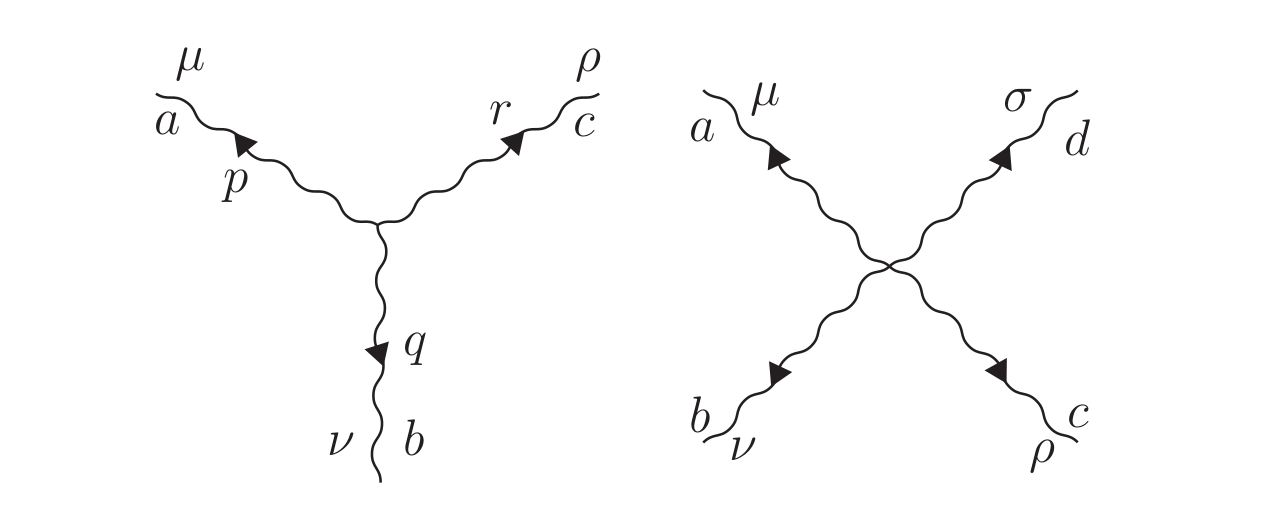
\includegraphics[height=4cm ,width=10.13cm]{QFT4/gluon_vertices.png}
	\caption{The three-gluon and four-gluon vertices in nonabelian gauge theory}
\end{figure}

\noindent
For loop calculations, we need to include the ghosts. The ghost lagrangian is
\[\mathcal{L}_{gh} = -\partial^{\mu}\overline{c}^c \partial_{\mu}c^c + gf^{abc}A^a_{\mu}\partial^{\mu}\overline{c}^b c^c\]
The ghost propagator is
\[D_F(k) = \frac{-i\delta^{ab}}{k^2-i\epsilon}\]
Because the ghosts are complex scalars, their propagators carry a charge arrow. 

\begin{figure}[!h]
	\centering
	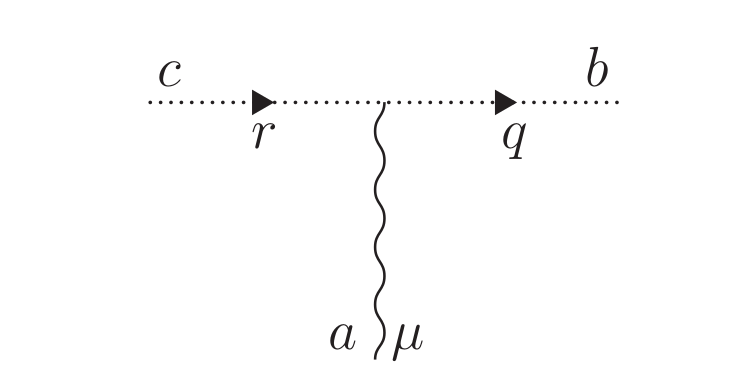
\includegraphics[height=4cm ,width=7.81cm]{QFT4/ggg_vertex.png}
	\caption{The ghost-ghost-gluon vertex in nonabelian gauge theory}
\end{figure}

\noindent
The ghost–ghost–gluon vertex factor is
\[iV^{abc}_{\mu}(-iq_{\mu}) = gf^{abc}a_{\mu}\]
If we include a quark coupled to the gluons, we have the quark lagrangian
\[\mathcal{L}_{q} = i\overline{\Psi}_{i}\slashed{D}_{ij}\Psi_{j} - m\overline{\Psi}_{i}\Psi_{i} = i\overline{\Psi}_{i}\slashed{\partial}\Psi_{i} - m\overline{\Psi}_{i}\Psi_{i} + gA^a_{\mu}\overline{\Psi}_{i} \gamma^{\mu} T^a_{ij} \Psi_j \]

\begin{figure}[!h]
	\centering
	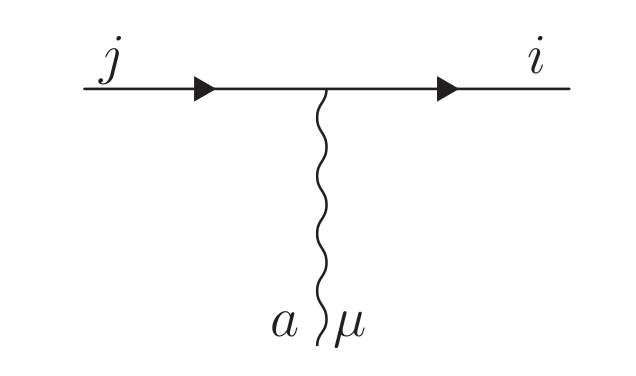
\includegraphics[height=3cm ,width=5.07cm]{QFT4/ffg_vertex.png}
	\caption{The quark-quark-gluon vertex in nonabelian gauge theory}
\end{figure}

\noindent
The quark propagator is
\[S_F(p)_{ij} = \frac{i(\slashed{p}-m)\delta_{ij}}{p^2+m^2 - i\epsilon}\]
The quark–quark–gluon vertex factor is
\[iV^{\mu a}_{ij} ig\gamma^{\mu}T^a_{ij}\]
















\end{document}
